\documentclass[11pt]{article}
\usepackage[a4paper,total={6in,8in}]{geometry}
\usepackage{cite,url}
\usepackage{tikz}
\usepackage{amsmath}
\usepackage{amsthm}
\usepackage{amssymb,amsfonts,nicefrac}
\usepackage{xspace}
\usepackage{color}
%\usepackage{url,hyperref}
%
\usepackage{bm}
\usepackage{bbm}
%\usepackage{times}
\usepackage{framed}%[framemethod=tikz]
\usepackage{enumerate}

\usepackage{algorithmic}
\usepackage{graphicx}
\usepackage{textcomp}
\usepackage{xcolor}
\usepackage{subfig}
\usepackage{array}
\usetikzlibrary{shapes,arrows}
\usepackage[ruled,linesnumbered,noend,algo2e]{algorithm2e}
\usepackage[lambda,
advantage,
operators,
sets, 
adversary, 
landau,
probability, 
notions, 
logic,
ff,
mm,
primitives, 
events, 
complexity, 
asymptotics, 
keys]{cryptocode}




\newtheorem{theorem}{Theorem}
\newtheorem{definition}{Definition}

\newtheorem{lemma}[theorem]{Lemma}

\newcommand{\mc}{\mathcal}
\title{Zero Knowledge Inner Product Argument}

\begin{document}
\maketitle


\section{Making Inner Product Zero Knowledge}
The inner prodcut protocol presented in the paper \cite[Section 3]{Bulletproofs}
presents a sound argument for the following relation:
\begin{align}\label{eq:ipa}
\{\big((P,v,\bm{g},\bm{h},g), (a,b)\big): P\in \GG, v\in \ZZ_p,
\bm{g},\bm{h}\in \GG^n, g\in \GG, a,b\in \ZZ_p^n, P=\bm{g}^a\bm{h}^b,\langle
a,b\rangle = v\}
\end{align}
In the above, $P$ is a binding commitment to vectors $a,b\in \ZZ_p^n$ purported
to satisfy the relation $\langle a,b \rangle = v$.
 
We will present a zero knowledge argument for inner product, where the prover
makes hiding and binding commitments to the vectors $a_L,a_R\in \ZZ_p^n$ and  
the inner product $\langle a_L,a_R\rangle$. Specifically, given $A\in \GG$,
$V\in \GG$ and $\bm{g},\bm{h}\in \GG^n$, $g,h\in \GG$, we give a zero knowledge
argument of knowledge of $a_L,a_R\in \ZZ_p^n$ and $v,\sigma,\delta\in \ZZ_p$
such that $A=h^\sigma\bm{g}^{a_L}\bm{h}^{a_R}$, $V=h^\delta g^v$ and
$\langle a_L,a_R\rangle = v$. We present the protocol below:

\begin{enumerate}[{\rm 1.}]
\item $\prover\leftrightarrow \verifier$: $A\in \GG$, $V\in \GG$,
$\bm{g},\bm{h}\in \GG^n$, $g,h\in \GG$. Remember that prover knows
$\sigma,\delta$ such that $A=h^\sigma\bm{g}^{a_L}\bm{h}^{a_R}$ and $V=h^\delta
g^{\langle a_L,a_R\rangle}$.  

\item $\prover\rightarrow \verifier$: Prover samples blinding vectors
$s_L,s_R\sample \ZZ_p^n$, $\rho\sample \ZZ_p$ and computes
$S=h^\rho\bm{g}^{s_L}\bm{h}^{s_R}$. The prover also computes the polynomial
$T(X) = \langle a_L + X.s_L, a_R + X.s_R \rangle = \langle a_L, a_R
\rangle + t_1X+t_2X^2$ for some $t_1,t_2\in \ZZ_p$. The prover computes
commitments $T_i=h^{\tau_i}g^{t_i}$ to the coefficients $t_i$ for $i=1,2$. The
prover sends $T_1,T_2$ to the verifier, thus committing to the polynomial
$T$.


\item $\verifier\rightarrow \prover$: Verifier samples $x\sample
\ZZ_p\backslash \{0\}$ and sends it to the prover.

\item $\prover\rightarrow \verifier$: The prover computes $\hat{l}=a_L+x.s_L$,
$\hat{r}=a_R+x.s_R$, $\hat{t}=T(x)=\langle \hat{l},\hat{r}\rangle$,
$P=\bm{g}^{\hat{l}}\bm{h}^{\hat{r}}$, $\mu=\sigma+\rho x$ and $\tau_x = \delta
+ \tau_1 x + \tau_2x^2$. The prover sends $P$, $\hat{t}, \mu$ and $\tau_x$ to the verifier.

\item The verifier proceeds as:
  \begin{itemize}
    \item Checks $h^{\tau_x}g^{\hat{t}} = V.T_1^x.T_2^{x^2}$ to check the
correct evaluation of the committed polynomial $T$ at $x$.
    \item Checks $A.S^x=h^\mu.P$.
    \item Runs the sound argument \eqref{eq:ipa} on $(P,\hat{t},\bm{g},\bm{h},g)$ with the prover.
  \end{itemize}
  The verifier accepts if the checks succeed and the inner product argument
accepts.
\end{enumerate}

\subsection{Completeness}
Let us argue the completeness of the above protocol. For honestly computed
values, the first check succeeds as shown below:
\begin{align*}
h^{\tau_x}g^{\hat{t}} &= h^{\delta + \tau_1x + \tau_2x^2}.
                            g^{\langle a_L, a_R \rangle + t_1x + t_2x^2} \\
&= h^\delta.h^{\tau_1x}.h^{\tau_2x^2}.g^{\langle a_L, a_R \rangle}.
  g^{t_1x}.g^{t_2x^2} \\
&= (h^\delta.g^{\langle a_L, a_R
\rangle}).(h^{\tau_1}g^{t_1})^x.(h^{\tau_2}g^{t_2})^{x^2} \\
&= V.T_1^x.T_2^{x^2} \qed
\end{align*}
Similarly the second check can be verified as:
\begin{align*}
A.S^x &= h^\sigma\bm{g}^{a_L}\bm{h}^{a_R}.(h^\rho\bm{g}^{s_L}\bm{h}^{s_R})^x \\
&= h^{\sigma + \rho x}.\bm{g}^{a_L + x.s_L}.\bm{h}^{a_R + x.s_R} \\
&= h^{\mu}.P \qed
\end{align*}
Finally, since the prover knows $\hat{l}=a_L+x.s_L$ and $\hat{r}=a_R+x.s_R$
such that $\hat{t}=\langle \hat{l},\hat{r} \rangle$ and
$P=\bm{g}^{\hat{l}}\bm{h}^{\hat{r}}$, by the completeness property of the inner
product argument, the verifier accepts in the inner product subprotocol. This
proves the completeness of the overall protocol. 

\section{Zero Knowledge}
Concretely, the transcript $\mc{T}$ consists of messages
$(x,T_1,T_2,P,S,\hat{t},\mu,\tau_x,\mc{T}_{in})$ where $\mc{T}_{in}$ denotes the
transcript of the inner product argument used as the subprotocol. We remove the
variables $S$ and $T_2$ from the transcript as these can be determinded from
verification equations, given the values of other variables in the transcript.
Thus we write $\mc{T}=(x,P,\hat{t},T_1,\mu,\tau_x,\mc{T}_{in})$. Note that the
distribution of the transcript depends on ``internal'' sampled variables
$s_L,s_R,\rho,\tau_1,\tau_2$ by the prover. We illustrate the dependence
pictorially in Figure \ref{fig:tg}. We also notice that $P,\hat{t}$ are
completely determined by $\hat{l},\hat{r}$. So we re-define our transcript to
be $(x,\hat{l},\hat{r},T_1,\mu,\tau_x)$ for the purpose of showing
zero-knowledge (note that including $\hat{l},\hat{r}$ in the actual transcript
would have made the argument size linear). Let $\Lambda =
(s_L,s_R,\rho,\tau_1,\tau_2)$ denote the variables in top row in Fig
\ref{fig:tg}, each of which is picked uniformly from its domain. The choices of
$\Lambda$ forms the probability space over which the transcript is defined.
Now we can
write the distribution of the transcript in an honest execution of the protocol
as:
\begin{align}\label{eq:factor}
p(x,\hat{l},\hat{r},T_1,\mu,\tau_x) &= p(x)\times p(\hat{l}|x)\times p(\hat{r}|\hat{l},x)\times p(T_1|\hat{l},\hat{r},x) \nonumber \\ 
&\quad \times p(\mu|T_1,\hat{l},\hat{r},x)\times
  p(\tau_x|\mu,T_1,\hat{l},\hat{r},x)
\end{align}

Now $\hat{l} = a_L + x.s_L$ and since $s_L$ is picked
uniformly at random, we have
$p(\hat{l}|x)=p(\hat{l})$ where $p(\hat{l})$ denotes the uniform distribution
over vectors in $\ZZ_p^n$. Similarly $p(\hat{r}|\hat{l},x)=p(\hat{r})$ as
$\hat{r}=a_R + x.s_R$ where $s_R$ is picked uniformly and independently of
$s_L$. Continuing $p(T_1|\hat{r},\hat{l},x)=p(T_1)$ as $T_1$ depends on
$\tau_1$ which is picked independently of $\hat{l},\hat{r},x$. In a similar
vein, $\mu$ is independent of the preceeding variables as it is blinded by
$\rho$ which is picked independently of the preceeding variables, and $\tau_x$
is independent of preceeding variables due to $\tau_2$. Thus in an honest
execution of the protocol, the distribution of the transcript factorizes as the
uniform distribution over each of the variables. The simulator randomly picks
the elements of the transcript and uses the deterministic relations to compute
$P,\hat{t},T_2$ and $S$. Finally, the transcript for
the inner product sub-protocol depends on $\hat{l},\hat{r}$ (which are the
prover witness for that protocol), and hence can be simulated using $\hat{l}$
and $\hat{r}$. This proves perfect zero knowledge for the protocol.

\begin{figure}[t!]
\centering
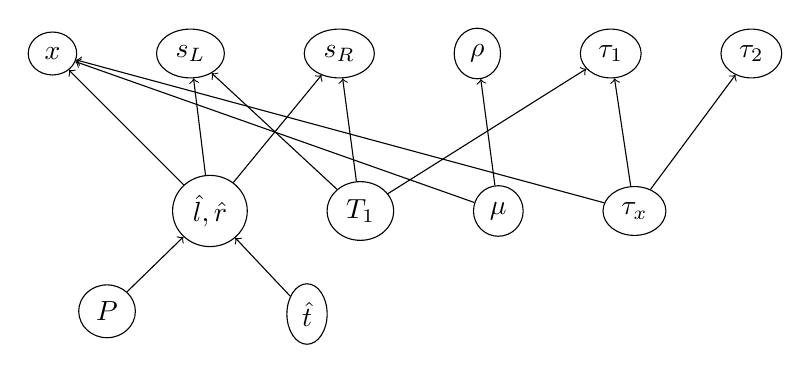
\begin{tikzpicture}[node distance=1cm]
\tikzset{events/.style = {ellipse, draw, align=center}};
\node (0,0) [events] (x) {$x$};
\node [events, right = of x] (sL) {$s_L$};
\node [events, right = of sL] (sR) {$s_R$};
\node [events, right = of sR] (rho) {$\rho$};
\node [events, right = of rho] (tau1) {$\tau_1$};
\node [events, right = of tau1] (tau2) {$\tau_2$};

\draw (2,-2) node[events] (hatLR) {$\hat{l},\hat{r}$};
\node [events, right = of hatLR] (T1) {$T_1$};
\node [events, right = of T1] (mu) {$\mu$};
\node [events, right = of mu] (taux) {$\tau_x$};

\node [events, below left = of hatLR] (P) {$P$};
\node [events, below right = of hatLR] (hatT) {$\hat{t}$};

\draw [<-] (x) -- (hatLR);
\draw [<-] (sL) -- (hatLR); 
\draw [<-] (sR) -- (hatLR);
\draw [<-] (sL) -- (T1);
\draw [<-]  (sR) -- (T1);
\draw [<-] (tau1) -- (T1);
\draw [<-] (x) -- (mu);
\draw [<-] (rho) -- (mu);
\draw [<-] (x) -- (taux);
\draw [<-] (tau1) -- (taux);
\draw [<-] (tau2) -- (taux);
\draw [<-] (hatLR) -- (P);
\draw [<-] (hatLR) -- (hatT);
\end{tikzpicture}
\caption{Transcript Graph}
\label{fig:tg}
\end{figure}
 

\bibliographystyle{plain}
\bibliography{references}
\end{document}


 

